\documentclass{article}
\usepackage[utf8]{vietnam}
\usepackage[vietnamese]{babel}
\usepackage{booktabs}
\usepackage{graphicx} % Required for inserting images
\usepackage{tikz}
\usepackage{enumerate}

\begin{document}
\tableofcontents

    
\section{Tọa độ đề các}



\begin{tikzpicture}
    \draw (0,0)--(3,3);
\end{tikzpicture}


\begin{tikzpicture}
    \draw (0,0) -- (3,0) 
                -- (3,4)
                -- (0,4)
                -- cycle;
\end{tikzpicture}

\section{Tọa độ cực}

\textbf{cứ theo góc, bán kính}
\hspace{3cm}

\begin{tikzpicture}
    \draw (0:2)--(45:2)
        -- (90:2) -- (135:2)
        -- (180:2) -- (225:2)
        -- (270:2) -- (315:2) -- cycle;
\end{tikzpicture}

nên dùng khi vẽ hình lỗi lõm

\section{Tọa độ tương đối: tịnh tiến đồ thị theo vector dùng khi vẽ cạnh}
\begin{tikzpicture}
    \draw (0,0) --++ (2, 0)--++(0,2) --++ (3,0);
\end{tikzpicture}


\begin{tikzpicture}
    \draw (0,0) -- (2, 0) -- (0,2);
\end{tikzpicture}

\subsection{rectangle}

\begin{tikzpicture}
    \draw (-2,-1) rectangle (2,1);
\end{tikzpicture}

\subsection{Đường tròn, elip}

\begin{tikzpicture}
    \draw (0,0) circle [radius = 2];    
\end{tikzpicture}
vẽ đường tròn có tâm và bán kính

\begin{tikzpicture}
    \draw (0,0) circle [ x radius = 2, y radius = 1];
\end{tikzpicture}

\subsection{cung tròn, cung elip}
\begin{tikzpicture}
    \draw (0,0) arc [radius =2, start angle = 0, end angle =135];
\end{tikzpicture}
Tương tự đối với elip

\section{Node}

\begin{tikzpicture}
    \draw (0,0) node {A}
    -- (0,1) node {B}
    -- (1,0) node {C};
\end{tikzpicture}

Thêm này vào thì ko bị đè nữa
\begin{tikzpicture}
    \draw (0,0) node[fill = white] {A}
    --(1,0) node[fill = lime] {B}
    --(0,1) node[fill = lime] {C};
    
\end{tikzpicture}
Hoặc thay đổi vị trí của node

\begin{figure}
    \centering
    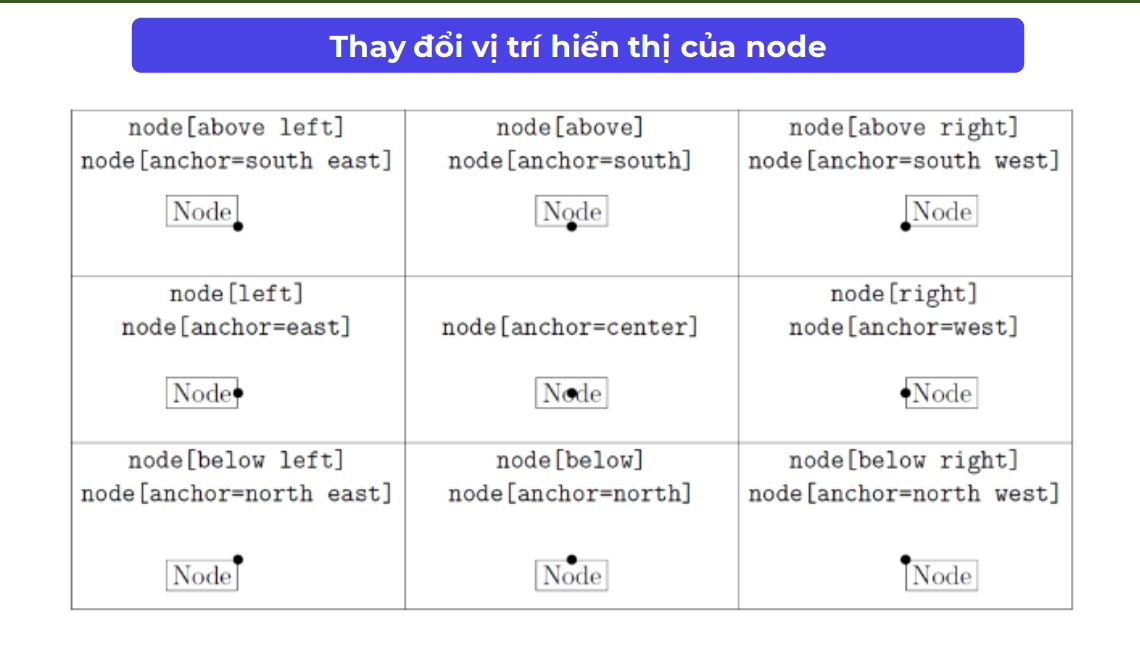
\includegraphics[scale = 0.6]{anh/node.png}
    \caption{Caption}
\end{figure}

\begin{figure}
    \centering
    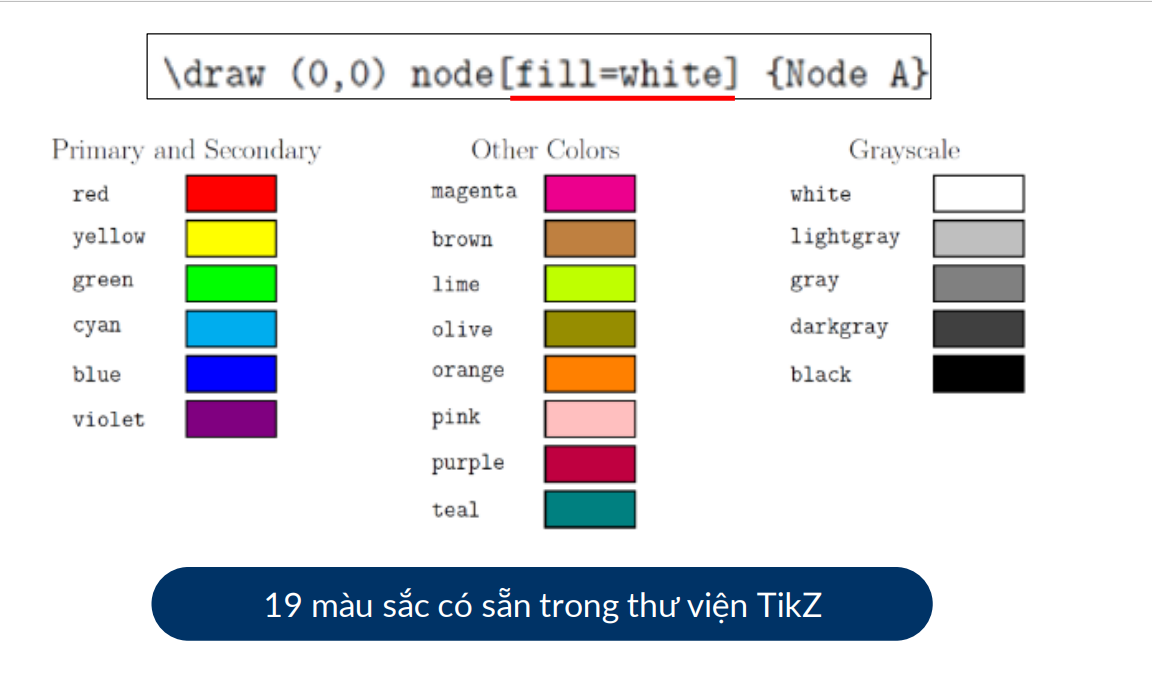
\includegraphics[scale = 0.6]{anh/color.png}
    \caption{Caption}
\end{figure}

\subsection{Tô màu hình vẽ}
\begin{tikzpicture}
    \draw[fill = yellow] (0,0)--(4,0)--(0,4) -- (4,4);
\end{tikzpicture}

Nếu hình không kín, lệnh fill sẽ tự động nối điểm đầu và 
điểm cuối nhưng không hiển thị đoạn thẳng đó

\section{Vẽ mũi tên}
\begin{tikzpicture}
    \draw[->] (0,0)--(1,1);
    \draw[<-] (2,2) -- (2,0);
    \draw[<->] (1,2) -- (2,1);
    \draw[<->>] (3,2) -- (2,4);
    \draw[<<->>] (4,2) -- (2,3);
    \draw[<>-><] (1,2) -- (2,-1);
    
\end{tikzpicture}

\section{Thao tác với hình khối}

\begin{tikzpicture}
    \draw (0,0) -| (6,2);
    
\end{tikzpicture}

\begin{tikzpicture}
    \draw (0,0) |- (3,5);
\end{tikzpicture}

Đường cong

\begin{tikzpicture}
    \draw (0,0) -- (5,0);
    \draw (0,0) to [bend left] (5,0);
\end{tikzpicture}

bend left trên, right dưới  mặc định độ cong là 30 độ, có thể tùy chỉnh

\begin{tikzpicture}
    \draw (0,0) to[out = 315, in = 135] (5,0);
\end{tikzpicture}

\section{tự tịnh tiến bằng lệnh shift}

\begin{tikzpicture}
    \draw (0,0) rectangle (1,1);
    \draw[shift = {(2,2)}] (0,0) rectangle (1,1);
\end{tikzpicture}

Tương tự với xshift là tăng kích thước x lên 2

Tương tự với yshift là tăng kích thước y lên 2

Tương tự với scale là tăng kích thước lên 2

Tương tự với rotato là xoay

\section{chèn ảnh vào node}

\begin{tikzpicture}
    \draw (0,0) node[draw]{
    \begin{tabular}{c|c}
         1& 1 \\
         \cmidrule{1-2}\\
         1&1 
    \end{tabular}
    };
\end{tikzpicture}


\begin{tikzpicture}
    \draw (5,5) node{
        
\includegraphics[scale = 0.1]{anh/ghost.png}
    };
\end{tikzpicture}

tương tự đối với biểu thức, boxtext....


\section{vẽ đồ thị}
\begin{tikzpicture}
    \draw[ultra thin,gray] (-4,-1) grid (4,5);
    \draw[<->] (-4.5,0) -- (4.5,0) node[right] {$x$};
    \draw[<->] (0, -4.5) -- (0,4.5) node[right] {$y$};
    % \clip (-4,1)--(4,5);
    \begin{scope}
        \clip (-4,-1)rectangle(4,5);
        \draw[domain = -3:3, variable = \x, samples =50, smooth,blue,thick] plot ({\x},{(\x)^2});
        
    \end{scope}
    \draw (-3,2) node[draw,blue,fill = white] {f(x) = $x^2$};
    \draw[red, fill = red] (2,4) circle [radius = 1mm] node[black, right] {(2,4)};
    \draw[red, dashed] (0,4) node[black, left]{a};
    \draw[red, dashed] (2,0) node[black, left]{b};
\end{tikzpicture}



Trong đó:
\begin{enumerate}
    \item domain: miền vẽ
    \item samples: số điểm vẽ(càng nhiều càng tốt, mặc định 50)
    \item smooth: cho đồ thị mượt hơn
    \item plot: lệnh vẽ đồ thị
    \item clip: dùng để cắt trong môi trường scope
\end{enumerate}

\begin{tikzpicture}
    \coordinate (A) at (1,1);
    \coordinate (B) at (2,2);
    \coordinate (C) at (4,3);
    \coordinate (D) at (1,4);
    \draw (A)--(B)--(C)--(D);   
\end{tikzpicture}

\section{Vòng lặp}


\end{document}
